\documentclass{article}

\usepackage[preprint]{neurips_2024}

\usepackage[utf8]{inputenc}
\usepackage[T1]{fontenc}
\usepackage{hyperref}
\usepackage{url}
\usepackage{booktabs}
\usepackage{amsfonts}
\usepackage{amsmath,amssymb}
\usepackage{nicefrac}
\usepackage{xcolor}
\usepackage{graphicx}
\usepackage{algorithm}
\usepackage{algorithmic}
\usepackage{float}
\usepackage{subcaption}
\usepackage{multirow}
\usepackage{bm}
\usepackage{pifont}

\raggedbottom
\setlength{\emergencystretch}{3em}
\hbadness=10000
\vbadness=10000

\newcommand{\model}{\textsc{NeuronSpark}}
\newcommand{\vpost}{V_{\text{post}}}
\newcommand{\vpre}{V_{\text{pre}}}
\newcommand{\vth}{V_{\text{th}}}
\newcommand{\vmin}{V_{\text{min}}}
\newcommand{\Expect}{\mathbb{E}}
\newcommand{\R}{\mathbb{R}}

\title{\model{}: A Spiking Neural Network Language Model with Selective State Space Dynamics}

\author{
  Zhengzheng Tang \\
  Boston University \\
  \texttt{zztangbu@bu.edu}
}

\begin{document}

\maketitle

% ============================================================
\begin{abstract}
We investigate whether large-scale language modeling can be achieved with a fully spiking backbone, without distillation from pretrained Transformers. This question is motivated by the need for architectures that preserve language modeling capacity while offering a clearer path to energy-efficient neuromorphic deployment. We present \model{}, a 0.9B-parameter spiking language model trained from random initialization via next-token prediction and surrogate-gradient optimization. The architecture combines selective state-space SNN blocks with input-dependent modulation of membrane decay, input gain, and firing threshold, leakage-current activation as the default inter-layer signal, and PonderNet-based adaptive timesteps for token-wise dynamic computation. It further incorporates fused Triton PLIF kernels and stabilization techniques, including residual centering, lateral-inhibition normalization, and natural-gradient compensation. Importantly, inter-layer communication is carried primarily by floating-point leakage-current signals rather than a pure binary spike stream; binary spikes are retained as internal firing events that shape membrane-state evolution. Under a constrained budget (approximately 1.4B pretraining tokens from a 10B-token Chinese corpus and approximately 6.5K SFT steps over 3.5M instruction samples), \model{}-0.9B reaches a pretraining loss of 3.6 and exhibits early multi-turn dialogue behavior after supervised fine-tuning. These results provide evidence that end-to-end language modeling with a pure SNN architecture is feasible at this scale.
\end{abstract}

% ============================================================
\section{Introduction}
\label{sec:intro}

Large language models (LLMs) based on Transformers~\citep{vaswani2017attention} have achieved remarkable success across natural language processing tasks.
However, their quadratic attention mechanism and dense floating-point computation raise fundamental questions about computational efficiency and biological plausibility.
Meanwhile, spiking neural networks (SNNs)~\citep{maass1997networks} --- the ``third generation'' of neural networks --- process information through discrete spikes and temporal dynamics, offering potential advantages in energy efficiency and neuromorphic hardware deployment.

Despite significant progress in SNN-based vision models, SNN language modeling remains underdeveloped.
This gap is important because language is a central benchmark for general sequence modeling; without evidence at language-model scale, claims about SNNs as a practical alternative to dense Transformer computation remain limited.
Existing approaches such as SpikeGPT~\citep{zhu2024spikegpt}, SpikingBERT~\citep{bal2024spikingbert}, and SpikeBERT~\citep{lv2023spikebert} either rely on distillation from pretrained Transformers, retain non-spiking components in critical stages, or remain at relatively small model scale.
Consequently, the field still lacks a clear answer to the following question: \emph{Can a pure SNN architecture learn language from random initialization at meaningful scale under standard next-token training?}

In this work, we address this gap by introducing \model{}, a 0.9B-parameter SNN language model trained from random initialization.
Given the available compute budget (8$\times$ RTX 4090 GPUs), we train on approximately $\sim$1.4B tokens from a 10B-token corpus; despite this constraint, the model exhibits non-trivial language generation and dialogue behavior.
Our key technical insight is that the membrane potential dynamics of Leaky Integrate-and-Fire (LIF) neurons can be formulated as a selective state space model~\citep{gu2024mamba}, where the decay rate $\beta$, input gain $\alpha$, and firing threshold $\vth$ serve as input-dependent gating mechanisms analogous to Mamba's selection mechanism.
This perspective enables us to design an end-to-end spiking language architecture that is both trainable at scale and interpretable through the SSM lens. A key modeling choice is to treat layer-to-layer signals as floating-point leakage-current signals, while retaining 0/1 spikes as the internal neuronal event process; this distinction avoids the expressivity bottleneck of purely binary inter-layer communication.

\paragraph{Contributions.}
\begin{enumerate}
    \item We propose the \textbf{Selective State Space SNN Block} with 7 parallel projection paths, computing dynamic $\beta(t), \alpha(t), \vth(t)$ from input signals through learned modulation networks with structured initialization, establishing a formal SNN--SSM duality (Section~\ref{sec:snn-block}).
    \item We introduce \textbf{leakage-current activation} $(1-\beta)\cdot\vpost$ as the default inter-layer signal for PLIFNode boundaries, which naturally emphasizes fast-responding neurons and provides implicit temporal-scale weighting (Section~\ref{sec:leakage}).
    \item We design \textbf{PonderNet adaptive timesteps} at each sublayer, enabling per-token dynamic SNN computation depth with geometric-distribution weighting and ponder cost regularization (Section~\ref{sec:pondernet}).
    \item We develop \textbf{Triton-fused PLIF kernels} with per-element and row-parameter variants, performing the entire PLIF forward/backward (including surrogate gradient) in a single kernel launch (Section~\ref{sec:triton}).
    \item We introduce \textbf{residual centering} and \textbf{lateral inhibition normalization} as SNN-native stabilization techniques, along with a two-phase \textbf{natural gradient compensation} for modulation parameters (Sections~\ref{sec:residual-centering}--\ref{sec:natural-gradient}).
    \item We train and release \model{}-0.9B under a constrained data budget, and provide evidence that a pure SNN can acquire non-trivial language modeling ability from random initialization (Section~\ref{sec:experiments}).
\end{enumerate}

Collectively, these contributions target a single bottleneck in prior work: the lack of a scalable, end-to-end spiking recipe for language modeling that is both theoretically grounded and practically trainable.

\begin{figure}[t]
    \centering
    
\includegraphics[width=\textwidth]{figures/Architrcture.png}
    \caption{\model{} architecture overview.
    The residual stream carries continuous values $\mathbf{h}$; PLIFLeak denotes PLIF neurons with leakage activation $(1-\beta)\cdot\vpost$.
    PonderNet aggregation (applied per sublayer) collapses $K$ frames per token with learned geometric-distribution weights.
    Inter-layer communication uses floating-point leakage-current signals; binary spikes are internal firing events rather than the default layer-to-layer representation.
    The decode stage uses uniform $K$-frame mean.
    Residual centering (subtract per-token mean) is applied before each residual addition.}
    \label{fig:architecture}
\end{figure}



% ============================================================
\section{Related Work}
\label{sec:related}

\paragraph{Spiking Neural Networks for Language.}
Prior work can be grouped by the specific gap it leaves unaddressed. \textbf{Distillation dependence}: SpikingBERT~\citep{bal2024spikingbert} and SpikeBERT~\citep{lv2023spikebert} transfer representations from pretrained ANN/Transformer models, which reduces evidence that language competence can emerge from fully spiking training dynamics. \textbf{Partial spiking pipelines}: SpikeGPT~\citep{zhu2024spikegpt} demonstrates generative behavior with spike-based hidden computation, but still retains non-spiking components (e.g., embedding/output stages), leaving end-to-end spiking feasibility unresolved. \textbf{Scale limitations}: existing studies are typically limited to $\leq$216M parameters, well below contemporary language-model regimes. Our work targets these three gaps jointly by training a 0.9B model from random initialization with standard next-token prediction and spiking dynamics throughout the core sequence-processing stack.

\paragraph{State Space Models.}
Structured State Spaces (S4)~\citep{gu2022efficiently} introduced efficient linear recurrence for sequence modeling.
Mamba~\citep{gu2024mamba} added input-dependent selection, achieving Transformer-competitive performance.
Mamba-2~\citep{dao2024transformers} established a formal duality between SSMs and attention.
We observe that SNN membrane dynamics $V[t] = \beta(t) \cdot V[t-1] + \alpha(t) \cdot I[t]$ are structurally identical to the selective SSM recurrence, with $\beta$ as the decay coefficient and $\alpha$ as the input gate.
The spike-and-reset mechanism adds a discrete nonlinearity absent in continuous SSMs.

\paragraph{Adaptive Computation.}
Adaptive Computation Time (ACT)~\citep{graves2016adaptive} allows networks to vary computation per input.
PonderNet~\citep{banino2021pondernet} improved upon ACT with a geometric distribution prior.
We apply PonderNet at the SNN timestep level within each sublayer: the $K$ frames per token are aggregated with learned halt probabilities, enabling different tokens to use 1 to $K_{\max}$ effective SNN steps.

\paragraph{Surrogate Gradient Training.}
The non-differentiability of spike generation ($\Theta(V - \vth)$) is addressed by surrogate gradient methods~\citep{neftci2019surrogate, zenke2021remarkable}, which replace the Heaviside derivative with smooth approximations.
\model{} uses Sigmoid surrogate gradients ($\alpha=4.0$) throughout, implemented in the SpikingJelly framework~\citep{fang2023spikingjelly}, with custom Triton kernels that fuse the surrogate computation into the sequential scan.

% ============================================================
\section{Architecture}
\label{sec:arch}

This section is organized around one central method question: how to make a pure SNN language model simultaneously expressive, trainable, and scalable. Our design follows a four-step logic: (1) define a stable neuron-level state update, (2) choose an inter-layer signal that avoids binary-communication bottlenecks, (3) build a selective sequence block on top of that signal, and (4) add system-level training stabilizers so optimization remains tractable at 0.9B scale.

\subsection{Overview}
\label{sec:overview}

\model{} follows a three-stage pipeline (Figure~\ref{fig:architecture}):
\textbf{(1)~Encode}: Token IDs $\to$ embedding ($D$-dim) $\to$ repeat $K$ times, producing a $(T{\cdot}K, B, D)$ tensor. Gradients flow directly through embedding; the output head reuses the embedding matrix (weight tying~\citep{press2017using}).
\textbf{(2)~SNN Forward}: $L{=}20$ decoder layers with gradient checkpointing, each containing an SNNBlock (attention analogue) and an SNNFFN (MLP analogue), with PonderNet adaptive $K$-frame aggregation. All neuron states reset per sequence.
\textbf{(3)~Decode}: RMSNorm~\citep{zhang2019root} $\to$ output PLIFNode (leakage) $\to$ $K$-frame uniform mean $\to$ projection $\to$ lateral inhibition~\citep{carandini2012normalization} $\to$ tied head $\to$ logits.

Each decoder layer follows a Pre-LN residual pattern matching Qwen3/LLaMA~\citep{touvron2023llama, yang2025qwen3}:
\begin{align}
    \mathbf{h} &\leftarrow \mathbf{h} + \text{center}\big(\text{OutProj}\big(\text{PonderAgg}\big(\text{SNNBlock}\big(\text{PLIFLeak}\big(\text{RMSNorm}(\mathbf{h})\big)\big)\big)\big)\big) \label{eq:layer-block} \\
    \mathbf{h} &\leftarrow \mathbf{h} + \text{center}\big(\text{OutProj}\big(\text{PonderAgg}\big(\text{SNNFFN}\big(\text{PLIFLeak}\big(\text{RMSNorm}(\mathbf{h})\big)\big)\big)\big)\big) \label{eq:layer-ffn}
\end{align}
where $\text{center}(\mathbf{x}) = \mathbf{x} - \text{mean}(\mathbf{x})$ is residual centering (Section~\ref{sec:residual-centering}).
The residual stream $\mathbf{h} \in \R^{TK \times B \times D}$ carries continuous values throughout; only the SNN sublayers operate on spike/membrane dynamics.

The remainder of this section instantiates this logic in order: PLIF dynamics define the base state transition, leakage-current activation defines the default inter-layer representation, SNNBlock/SNNFFN define sequence computation, and the final subsections describe optimization-oriented stabilizers.


\subsection{PLIF Neuron Dynamics (Mechanism)}
\label{sec:plif}

All neurons in \model{} follow the Parametric Leaky Integrate-and-Fire (PLIF) model~\citep{fang2021incorporating}. This subsection provides the dynamical foundation on which all later architectural choices are built.
We distinguish two variants:

\paragraph{PLIFNode (fixed parameters).}
Used at layer boundaries (input neurons, gate/up neurons, output neuron).
Each has $D$-dimensional (or $D_{\text{ff}}$-dimensional) learnable parameters:
\begin{align}
    \vpre[t] &= \beta \cdot \vpost[t-1] + (1-\beta) \cdot x[t] \label{eq:plif-charge} \\
    s[t] &= \Theta(\vpre[t] - \vth) \label{eq:plif-fire} \\
    \vpost[t] &= \vpre[t] - \vth \cdot s[t] \label{eq:plif-reset}
\end{align}
where $\beta = \sigma(w) \in (0,1)$ with $w \sim \mathcal{N}(\text{logit}(1 - 1/\tau_0),\; 0.5)$ and $\vth \sim \mathcal{U}(0.5 v_0,\; 1.5 v_0)$.
The random initialization creates diversity across dimensions: different neurons have different time constants and firing sensitivities.
Equation~\eqref{eq:plif-reset} implements \emph{soft reset}: the membrane potential is reduced by $\vth$ upon firing, preserving residual charge.

\paragraph{SelectivePLIFNode (dynamic parameters).}
Used inside SNNBlock for $D \cdot N$ hidden neurons.
Parameters $\beta(t), \alpha(t), \vth(t)$ are computed per-step from the input (Section~\ref{sec:snn-block}):
\begin{align}
    V[t] &= \beta(t) \cdot V[t-1] + \alpha(t) \cdot I[t] \label{eq:selective-charge} \\
    s[t] &= \Theta(V[t] - \vth(t)) \label{eq:selective-fire} \\
    V[t] &\mathrel{-}= \vth(t) \cdot s[t] \label{eq:selective-reset}
\end{align}
This is structurally identical to Mamba's selective SSM recurrence $h[t] = \bar{A}(t) \cdot h[t-1] + \bar{B}(t) \cdot x[t]$, with the addition of the spike-and-reset nonlinearity.

\subsection{Membrane Potential Leakage Activation (Signal)}
\label{sec:leakage}

A critical design choice is the signal transmitted between components. This is the key bridge from neuron dynamics to network-level information flow.
Standard SNN practice uses binary spikes $s[t] \in \{0,1\}$, but this severely limits gradient flow through the surrogate function's narrow support.
An alternative is the raw membrane potential $\vpost$, but this treats all neurons equally regardless of their temporal dynamics.

We use \textbf{leakage-current activation} as the default inter-layer signal. In other words, unless explicitly stated otherwise, downstream layers consume floating-point leakage-current signals (bioelectric-state proxies) rather than binary spikes:
\begin{equation}
    \text{leak}[t] = (1 - \beta) \cdot \vpost[t]
    \label{eq:leakage}
\end{equation}
This quantity is the amount of membrane potential that will \emph{dissipate} due to exponential decay before the next input arrives.
Biologically, it corresponds to the leak current through the membrane conductance~\citep{hodgkin1952quantitative, abbott1999lapicque}.

This leakage-current activation provides natural \textbf{temporal-scale weighting}:
neurons with large $(1-\beta)$ (fast dynamics, short memory) produce proportionally larger signals,
while neurons with small $(1-\beta)$ (slow dynamics, long memory) are implicitly attenuated.
This reweighting is applied at all PLIFNode outputs: input neurons (2 per layer), gate/up neurons in SNNFFN (2 per layer), and the output neuron.

The SelectivePLIFNode \emph{hidden} neurons inside SNNBlock output raw $\vpost$ rather than leakage, because $\beta(t)$ is dynamic (varies per step) and cannot be absorbed into a static downstream weight matrix.
This is a deliberate design choice: leakage scaling applies only at fixed-$\beta$ boundaries.

\subsection{Selective State Space SNN Block (Module)}
\label{sec:snn-block}

With neuron dynamics and inter-layer signaling fixed, we next define the core sequence module. The SNNBlock is the attention analogue, processing input through $D \cdot N$ hidden spiking neurons with input-dependent parameters.
It computes \textbf{seven parallel projections} from the input leakage signal --- six input projections and one output projection:

\paragraph{Input projections} ($D \to D \cdot N$ or $D \to D$):
\begin{align}
    \mathbf{I}[t] &= W_{\text{in}} \cdot \text{leak}[t] \in \R^{DN} \quad \text{(input current)} \label{eq:block-I} \\
    \beta(t) &= \sigma(W_\beta \cdot \text{leak}[t] + \mathbf{b}_\beta) \in (0,1)^{DN} \quad \text{(decay rate)} \label{eq:block-beta} \\
    \alpha(t) &= \text{softplus}(W_\alpha \cdot \text{leak}[t] + \mathbf{b}_\alpha) \in \R_+^{DN} \quad \text{(input gain)} \label{eq:block-alpha} \\
    \vth(t) &= \vmin + |W_{\text{th}} \cdot \text{leak}[t] + \mathbf{b}_{\text{th}}| \in [\vmin, \infty)^{DN} \quad \text{(threshold)} \label{eq:block-vth} \\
    \mathbf{g}[t] &= \sigma(W_{\text{gate}} \cdot \text{leak}[t]) \in (0,1)^D \quad \text{(output gate)} \label{eq:block-gate} \\
    \mathbf{I}_{\text{skip}}[t] &= W_{\text{skip}} \cdot \text{leak}[t] \in \R^D \quad \text{(skip connection)} \label{eq:block-skip}
\end{align}
The modulation projections $W_\beta, W_\alpha, W_{\text{th}}$ are initialized at $0.1\times$ the scale of $W_{\text{in}}$, ensuring that $\beta(t), \alpha(t), \vth(t)$ are dominated by their respective biases at the start of training, providing a stable initialization.

\paragraph{Hidden neuron dynamics.}
The $D \cdot N$ hidden neurons follow SelectivePLIF (Eqs.~\ref{eq:selective-charge}--\ref{eq:selective-reset}), computed via fused Triton PLIF kernels (Section~\ref{sec:triton}).

\paragraph{Output projection} ($D \cdot N \to D$):
\begin{equation}
    \text{out}[t] = W_{\text{out}} \cdot \vpost[t] \odot \mathbf{g}[t] + \mathbf{I}_{\text{skip}}[t]
    \label{eq:block-out}
\end{equation}
Note: the output uses $\vpost$ (not leakage) from the hidden neurons, because $\beta(t)$ is dynamic.
The gate $\mathbf{g}$ provides multiplicative control over which dimensions pass through.
The skip connection $\mathbf{I}_{\text{skip}}$ ensures gradient flow even when all hidden neurons are silent.

\paragraph{Structured initialization.}
The modulation biases $\mathbf{b}_\beta, \mathbf{b}_\alpha, \mathbf{b}_{\text{th}}$ receive carefully designed initialization (details in Appendix~\ref{app:init}):
$\mathbf{b}_\beta$ is logit-spaced across $N$ groups targeting $\beta \in [0.80, 0.99]$ (multi-timescale);
$\mathbf{b}_\alpha$ is initialized near $\text{softplus}^{-1}(1.0)$ so initial $\alpha \approx 1$;
$\mathbf{b}_{\text{th}}$ is calibrated from stationary variance $\sigma_V = \sqrt{p/3} \cdot \sqrt{1 - \beta^{2K}}$ with target firing rates 25\%--8\% across $N$ groups;
$W_{\text{in}}$ rows are scaled by $\sqrt{1 - \beta^2}$ per group;
$W_{\text{out}}$ columns are scaled by $1/\sqrt{p_{\text{fire}}}$ per group.

\subsection{SNN Feed-Forward Network}
\label{sec:snn-ffn}

The SNNFFN mirrors the SwiGLU MLP~\citep{touvron2023llama} with spiking neurons replacing the activation function:
\begin{align}
    \text{gate\_leak} &= (1-\beta_g) \cdot \vpost(\text{PLIF}_{\text{gate}}(W_{\text{gate}} \cdot \text{leak})) \label{eq:ffn-gate} \\
    \text{up\_leak} &= (1-\beta_u) \cdot \vpost(\text{PLIF}_{\text{up}}(W_{\text{up}} \cdot \text{leak})) \label{eq:ffn-up} \\
    \text{out} &= W_{\text{down}} \cdot (\text{gate\_leak} \odot \text{up\_leak}) + W_{\text{skip}} \cdot \text{leak} \label{eq:ffn-out}
\end{align}
The element-wise product of two leakage signals replaces $\text{SiLU}(x) \odot x$ gating in SwiGLU~\citep{shazeer2020glu}.
Both PLIF neurons provide implicit nonlinearity through the integrate-fire-reset cycle; their leakage outputs carry temporal dynamics that pure activation functions cannot express.
$W_{\text{down}}$ is initialized with $1/\sqrt{L}$ scaling to prevent gradient explosion through deep residual chains.

\subsection{PonderNet Adaptive Timesteps (Module)}
\label{sec:pondernet}

Each token is represented as $K$ SNN frames.
Rather than uniformly averaging all $K$ frames, we learn per-frame halt probabilities following PonderNet~\citep{banino2021pondernet}:
\begin{align}
    p_k &= \sigma(W_{\text{halt}} \cdot \text{frame}_k + b_{\text{halt}}) \in (0, 1) \label{eq:ponder-halt} \\
    S_k &= \textstyle\prod_{j=1}^{k-1} (1 - p_j) \quad \text{(survival probability)} \label{eq:ponder-survive} \\
    \lambda_k &= p_k \cdot S_k, \quad \hat{\lambda}_k = \lambda_k / \textstyle\sum_{k'} \lambda_{k'} \label{eq:ponder-lambda} \\
    \text{output} &= \textstyle\sum_k \hat{\lambda}_k \cdot \text{frame}_k, \quad \Expect[K] = \textstyle\sum_k k \cdot \hat{\lambda}_k \label{eq:ponder-agg}
\end{align}
$\Expect[K]$ serves as a ponder cost regularizer ($\lambda_{\text{ponder}} = 0.01$).
PonderNet is applied independently at each sublayer ($2L = 40$ aggregation points).
$W_{\text{halt}}$ is initialized with Xavier uniform $\times 0.01$ and $b_{\text{halt}} = -3.5$ ($\sigma(-3.5) \approx 0.03$), so PonderNet starts near-uniform and gradually specializes.

After aggregation, the result is projected through OutProj ($D \to D$, no bias), then broadcast back to $K$ frames for residual addition.

% ============================================================
\section{Stabilization and Efficient Implementation}
\label{sec:implementation}

\subsection{Residual Centering (Stabilizer)}
\label{sec:residual-centering}

Each sublayer's output projection is mean-subtracted before residual addition:
$\text{center}(\mathbf{x}) = \mathbf{x} - \frac{1}{D} \sum_{d=1}^{D} x_d$.
This eliminates DC drift that would otherwise accumulate across 20 residual layers.

\subsection{Lateral Inhibition Normalization (Stabilizer)}
\label{sec:lateral-inhibition}

The output layer uses \textbf{lateral inhibition} (divisive normalization):
$\text{LateralInhib}(\mathbf{h}) = \gamma \cdot \mathbf{h} / \sqrt{\frac{1}{D}\sum_d h_d^2 + \epsilon}$,
where $\gamma \in \R^D$ is a learnable gain.
This is mathematically equivalent to RMSNorm~\citep{zhang2019root} but corresponds to divisive normalization~\citep{carandini2012normalization}.
We implement it as a fused Triton kernel.

\subsection{Triton Fused PLIF Kernels (System)}
\label{sec:triton}

The PLIF recurrence involves a sequential scan that cannot be trivially parallelized due to spike-and-reset.
We implement two variants of fused Triton~\citep{tillet2019triton} kernels:

\textbf{Per-element kernel} (SelectivePLIFNode, dynamic $\beta[k], \vth[k]$): single-pass sequential scan with inline charge--fire--reset and Sigmoid surrogate gradient in the backward pass. All arithmetic in fp32 with bf16 storage.

\textbf{Row-parameter kernel} (PLIFNode, fixed $\beta, \vth$): parameters loaded once into registers, reducing global memory reads from 3 per step to 1, yielding $\sim$40\% speedup. Backward kernel accumulates $\nabla_\beta, \nabla_{\vth}$ in registers.

\textbf{CPU fallback}: 3-phase approach via Hillis-Steele parallel prefix scan~\citep{blelloch1990prefix, martin2018parallelizing}, spike fixed-point iteration, and surrogate gradient re-computation.

\subsection{Natural Gradient Compensation (Stabilizer)}
\label{sec:natural-gradient}

The modulation biases $\mathbf{b}_\beta, \mathbf{b}_\alpha, \mathbf{b}_{\text{th}}$ suffer from two gradient pathologies.
We apply compensation after gradient unscaling and before gradient clipping:

\textbf{Phase 1: Activation saturation.}
$\nabla_{b_\beta} \leftarrow \nabla_{b_\beta} / \max(\beta(1-\beta),\; 1/C_{\max})$, effectively performing gradient descent in $\beta$-space.
Similarly for $\alpha$: $\nabla_{b_\alpha} \leftarrow \nabla_{b_\alpha} / \max(\sigma(b_\alpha), 0.1)$.

\textbf{Phase 2: Cross-layer equalization.}
For each modulation parameter type, normalize per-layer gradient norms to the geometric mean:
$\nabla_{\text{layer}_i} \leftarrow \nabla_{\text{layer}_i} \cdot \text{GeoMean}(\|\nabla_1\|, \ldots, \|\nabla_L\|) / \|\nabla_i\|$.

% ============================================================
\section{Experiments}
\label{sec:experiments}

\subsection{Setup}

\paragraph{Model configuration.}
\model{}-0.9B: $D=896$, $N=8$, $K=16$, $L=20$, $D_{\text{ff}}=2688$, 6144-token BPE~\citep{sennrich2016neural} vocabulary, 874M parameters.

\paragraph{Datasets.}
\emph{Pretraining}: Seq-Monkey~\citep{seqmonkey2023} ($\sim$29M samples, $\sim$10B tokens).
\emph{SFT}: BelleGroup train\_3.5M\_CN~\citep{bellegroup2023} ($\sim$3.5M conversations).

\paragraph{Compute constraints.}
All training was conducted on 8$\times$ NVIDIA RTX 4090 GPUs.
Due to limited compute, we train on \textbf{small subsets}:

\begin{table}[H]
\centering
\small
\caption{Dataset utilization.}
\label{tab:data}
\begin{tabular}{lccc}
\toprule
\textbf{Stage} & \textbf{Full Dataset} & \textbf{Actual Used} & \textbf{Fraction} \\
\midrule
Pretrain & $\sim$10B tokens & 85K steps ($\sim$1.4B tokens) & $\sim$14\% \\
SFT & $\sim$3.5M conversations & 6.5K steps ($\sim$42K samples) & $\sim$1.2\% \\
\bottomrule
\end{tabular}
\end{table}

\paragraph{Training details.}
Pretraining: Adam~\citep{loshchilov2019decoupled}, peak lr$=2{\times}10^{-4}$, 1000-step warmup, cosine decay, gradient accumulation 8, effective batch 64, bfloat16~\citep{micikevicius2018mixed}, gradient checkpointing~\citep{chen2016training}.
Neuron parameters receive $10\times$ base lr.
SFT: AdamW (lr$=5{\times}10^{-5}$, weight decay 0.01), training only on assistant response tokens.

\subsection{Results}

\begin{table}[H]
\centering
\small
\caption{Training results for \model{}-0.9B.}
\label{tab:results}
\begin{tabular}{lcc}
\toprule
\textbf{Metric} & \textbf{Pretrain} & \textbf{SFT} \\
\midrule
Training loss & 3.6 & 2.1 \\
Parameters & \multicolumn{2}{c}{874M} \\
Training steps & 85,000 & 6,500 \\
Tokens seen & $\sim$1.4B & $\sim$0.4B \\
Hardware & \multicolumn{2}{c}{8$\times$ NVIDIA RTX 4090} \\
\bottomrule
\end{tabular}
\end{table}

\begin{figure}[t]
    \centering
    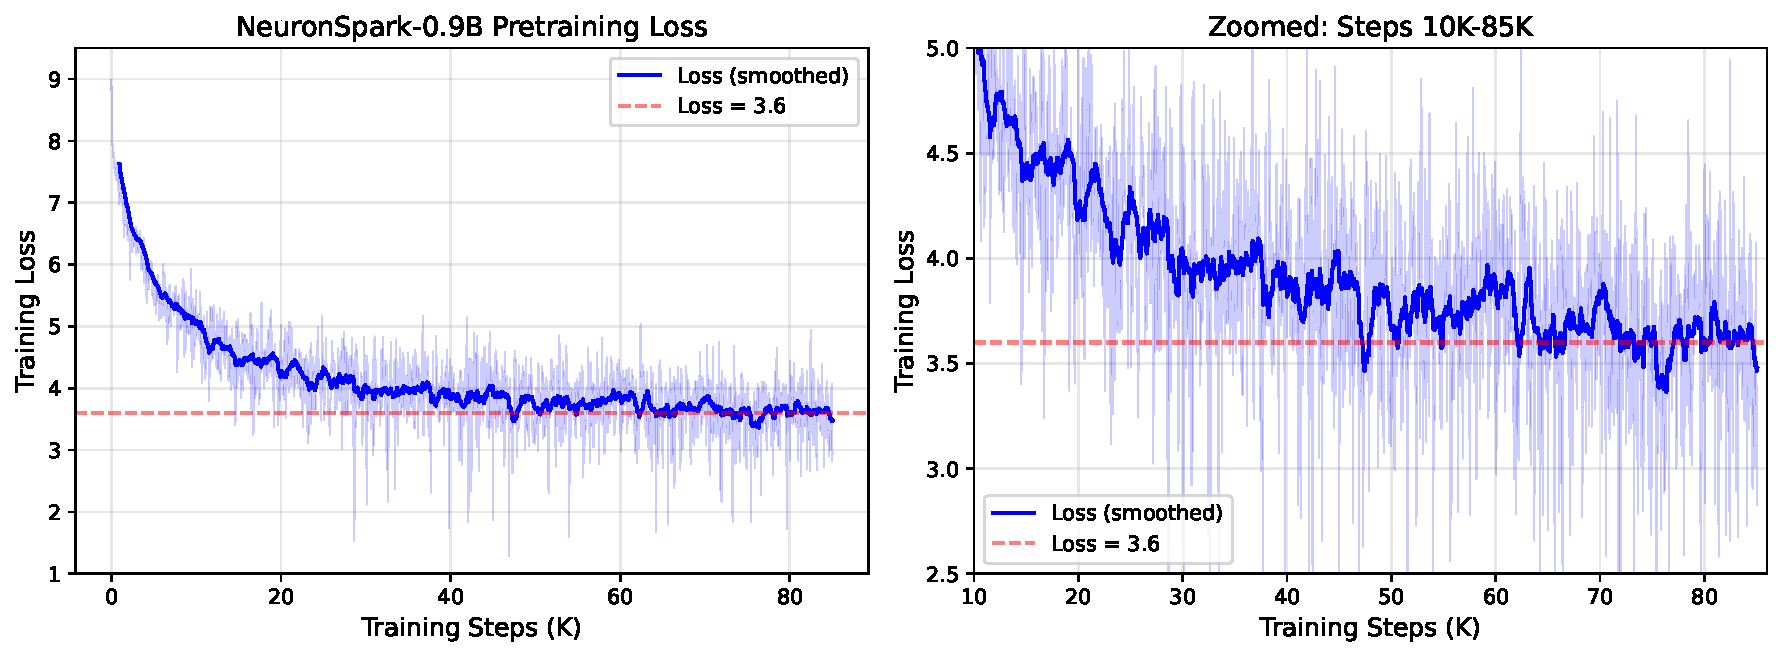
\includegraphics[width=\textwidth]{figures/loss_curve.pdf}
    \caption{Pretraining loss curve over 85K steps ($\sim$1.4B tokens). Loss decreases from 9.0 to $\sim$3.5.
    Training throughput: $\sim$960 tokens/sec on 8$\times$ RTX 4090 GPUs.}
    \label{fig:loss-curve}
\end{figure}

\paragraph{Qualitative evaluation.}
After SFT, the model demonstrates basic Chinese dialogue (translated; model outputs in Chinese):

\begin{quote}
\begin{tabular}{@{}l l@{}}
\textbf{Q:} What is the capital of China? & \textbf{A:} The capital of China is Beijing.\\
\textbf{Q:} Hello! & \textbf{A:} How can I help you?
\end{tabular}
\end{quote}

These observations suggest that a pure SNN architecture can support coherent language generation from random initialization, even under limited-data training.

\subsection{Architecture Ablation via Training Stability}
\label{sec:ablation}

During development, we explored multiple architectural variants (each trained 1K--12K steps).
Table~\ref{tab:ablation} summarizes 7 variants; Figure~\ref{fig:ablation} shows loss curves.

\begin{table}[H]
\centering
\scriptsize
\caption{Ablation variants. All stagnated above loss 7.0; only the final architecture reached 3.5.}
\label{tab:ablation}
\begin{tabular}{p{2.2cm}rrp{4cm}}
\toprule
\textbf{Variant} & \textbf{Steps} & \textbf{Loss} & \textbf{What Changed} \\
\midrule
\textbf{Final V1} & \textbf{85K} & \textbf{3.5} & \textbf{Full architecture} \\
\midrule
MPD-AGL + no Phase 2 & 4.8K & 7.21 & Adaptive surrogate gradient, removed cross-layer equalization \\
E[K] floor & 1.2K & 7.47 & Added minimum E[K] floor \\
Bounded $\alpha$ & 5.1K & 7.47 & Bounded gain multiplier \\
HC $\alpha$ (decoupled) & 3.7K & 7.44 & Separate $\alpha$ parameter \\
Sinkhorn health & 2.1K & 7.62\textsuperscript{$\dagger$} & Sinkhorn-projected health score \\
Cortical lateral & 4.1K & 7.66\textsuperscript{$\dagger$} & Cross-token causal spike propagation \\
No gradient sync & 0.6K & NaN & Missing gradient synchronization \\
\bottomrule
\multicolumn{4}{l}{\textsuperscript{$\dagger$}Diverged (loss $>$7.5).}
\end{tabular}
\end{table}

\begin{figure}[t]
    \centering
    
\includegraphics[width=\textwidth]{figures/ablation_runs.pdf}
    \caption{Training loss: final architecture (blue) vs.\ 9 ablation variants.
    None of the ablation variants achieves a loss below 7.0.}
    \label{fig:ablation}
\end{figure}

\subsection{Comparison with Existing SNN Language Models}

\begin{table}[H]
\centering
\small
\caption{Comparison with existing SNN language models.}
\label{tab:comparison}
\begin{tabular}{lccccc}
\toprule
\textbf{Model} & \textbf{Params} & \textbf{From Scratch} & \textbf{SNN Core} & \textbf{Generative} & \textbf{Dialogue} \\
\midrule
SpikeBERT & 110M & \ding{55} & \ding{51} & \ding{55} & \ding{55} \\
SpikingBERT & 110M & \ding{55} & \ding{51} & \ding{55} & \ding{55} \\
SpikeGPT & 216M & \ding{51} & \ding{51} & \ding{51} & \ding{55} \\
\textbf{\model{}-0.9B} & \textbf{874M} & \ding{51} & \ding{51} & \ding{51} & \ding{51} \\
\bottomrule
\end{tabular}
\end{table}

% ============================================================
\section{Discussion}
\label{sec:discussion}

Our central claim is that large-scale language modeling in a pure SNN regime is not only conceptually plausible but empirically attainable when the architectural design directly addresses the optimization and expressivity gaps left by prior SNN language studies.
Beyond feasibility, our interpretability analyses (Appendix~\ref{app:interpretability}) reveal that the trained model develops computational strategies with striking parallels to biological neural processing.

\paragraph{SNN--SSM duality.}
The selective PLIF dynamics establish a direct correspondence with Mamba's selective SSM:
$\beta(t) \leftrightarrow \bar{A}(t)$, $\alpha(t) \leftrightarrow \bar{B}(t)$, $V[t] \leftrightarrow h[t]$.
The spike-and-reset mechanism introduces a hard, input-dependent nonlinearity absent in continuous SSMs.

\paragraph{Biological interpretability: structure before semantics.}
Three complementary experiments (Appendix~\ref{app:interpretability}) paint a coherent picture of what the model learns and how it allocates neural resources:

\emph{(1)~Resource allocation mirrors syntactic role, not predictive difficulty.}
PonderNet assigns systematically fewer SNN steps to punctuation and function words than to content words (nouns, verbs, adjectives), mirroring how biological cortical circuits allocate differential processing effort based on stimulus structural complexity rather than statistical surprise~\citep{carandini2012normalization}.
Critically, E[K] is uncorrelated with token surprisal ($r = -0.12$ after excluding the BOS sentinel), confirming that adaptive computation is governed by syntactic role rather than prediction error --- a pattern consistent with neurolinguistic findings that neural processing load correlates more with syntactic complexity than with information-theoretic surprisal.

\emph{(2)~Hierarchical computation depth resembles cortical processing.}
Deeper layers allocate progressively more SNN timesteps (SNNBlock E[K] increases from $\sim$4 at layer~2 to $\sim$12.7 at layer~19), while SNNFFN E[K] remains stable ($\sim$7--8).
This asymmetry parallels the cortical hierarchy where higher-order areas exhibit longer temporal integration windows, and point-wise transformations (analogous to SNNFFN) saturate at a fixed processing depth.

\emph{(3)~Multi-timescale neuron specialization.}
The 143,360 hidden neurons self-organize into fast-responding ($\beta < 0.9$, 67.3\%) and slow-memory ($\beta \geq 0.9$, 32.7\%) populations, reminiscent of the coexistence of fast-spiking interneurons and regular-spiking pyramidal cells in biological cortex.

\emph{(4)~Structural competence without reasoning.}
The model achieves fluent Chinese generation (6/6 coherence) but fails at arithmetic (0/8), with E[K] flat across all task categories ($\sim$7.6).
This dissociation between structural fluency and reasoning ability, combined with the structure-driven (not difficulty-driven) computation allocation, suggests that the model has acquired a ``structural backbone'' of language --- analogous to early stages of biological language acquisition where grammatical patterns precede semantic understanding.
Continued training on more data would be needed to progress from structural pattern learning to genuine semantic reasoning.

\paragraph{Data efficiency.}
\model{} acquires basic language capabilities with $\sim$14\% of pretraining data and $\sim$1.2\% of SFT data.
The biological interpretability findings above suggest this efficiency may arise from the SNN architecture's inductive bias toward structural pattern extraction, though controlled Transformer baselines are needed to confirm this hypothesis.

\paragraph{Limitations.}
(1) 0.9B parameters, 512-token context. (2) No quantitative benchmarks (C-Eval, CMMLU) or Transformer baselines. (3) Chinese only. (4) Repetition artifacts and no reasoning capability. (5) Interpretability analyses are correlational, not causal.

\paragraph{Energy efficiency.}
The spike-based hidden computation may be amenable to deployment on neuromorphic platforms (e.g., Intel Loihi~\citep{davies2018loihi}), which could yield substantial energy savings. A rigorous quantitative evaluation remains future work.

% ============================================================
\section{Conclusion}
\label{sec:conclusion}

We presented \model{}, a 0.9B-parameter spiking language model that jointly addresses three persistent gaps in prior work: distillation dependence, partially non-spiking pipelines, and limited model scale.
By connecting SNN membrane dynamics to selective state space models and introducing leakage-current inter-layer signaling, PonderNet adaptive timesteps, fused Triton PLIF kernels, residual centering, lateral inhibition normalization, and natural-gradient compensation, we show that pure SNN architectures can learn non-trivial language behavior from random initialization under limited training data.

Beyond architectural feasibility, our interpretability analyses reveal that the trained model develops biologically plausible computational strategies: structure-driven (not difficulty-driven) resource allocation, hierarchical depth-dependent processing, multi-timescale neuron specialization, and a ``structure before semantics'' learning progression that parallels biological language acquisition.
These findings suggest that SNN architectures may offer not only energy-efficiency potential but also a path toward more interpretable language models grounded in neuroscience principles.

Code, weights, and training infrastructure are publicly available\footnote{Code: \url{https://github.com/Brain2nd/NeuronSpark}; HuggingFace: \url{https://huggingface.co/Brain2nd}; ModelScope: \url{https://modelscope.ai/organization/Brain2nd}.}.

% ============================================================
\bibliography{references}
\bibliographystyle{plainnat}

% ============================================================
\appendix

\section{Structured Initialization Details}
\label{app:init}

The SNNBlock modulation parameters require careful initialization.
We target $K_{\text{ref}} = 16$ steps and assumed input firing rate $p = 0.15$.

\textbf{Multi-timescale $\beta$}: $\beta_n = \text{linspace}(0.80, 0.99, N)$; bias $b_{\beta,\,n} = \log(\beta_n / (1 - \beta_n))$, repeated across $D$ channels with $\mathcal{N}(0, 0.1)$ perturbation.

\textbf{$\alpha$ near unity}: $b_\alpha \sim \mathcal{N}(0.5413, 0.1)$, giving $\alpha \approx 1.0$.

\textbf{Threshold calibration}: $\sigma_V(\beta) = \sqrt{p/3} \cdot \sqrt{1 - \beta^{2K_{\text{ref}}}}$; target firing rates $p_{\text{fire}} = \text{linspace}(0.25, 0.08, N)$; $V_{\text{th},n} = \sigma_V(\beta_n) \cdot \Phi^{-1}(1 - p_{\text{fire},n})$.

\textbf{$W_{\text{in}}$ scaling}: rows scaled by $\sqrt{1 - \beta_n^2}$ per group.
\textbf{$W_{\text{out}}$ balancing}: columns scaled by $1/\sqrt{p_{\text{fire},n}}$ (normalized to mean 1).

\section{Model Configuration}
\label{app:config}

\begin{table}[H]
\centering
\small
\caption{Detailed model configuration.}
\begin{tabular}{ll}
\toprule
Hidden dim ($D$) & 896 \\ State expansion ($N$) & 8 \\ Max SNN steps ($K$) & 16 \\
Layers ($L$) & 20 \\ FFN dim ($D_{\text{ff}}$) & 2688 \\ Vocab & 6144 \\ Context & 512 \\
Total params & 874M \\
\midrule
Surrogate & Sigmoid($\alpha$=4.0) \\ $\vmin$ & 0.1 \\ Neuron LR mult & 10$\times$ \\ Ponder weight & 0.01 \\
Output proj init & $0.02/\sqrt{2L}$ (GPT-2~\citep{radford2019language}) \\
\bottomrule
\end{tabular}
\end{table}

\section{Parameter Breakdown}
\label{app:params}

\begin{table}[H]
\centering
\small
\caption{Parameter breakdown. SNNBlock dominates (77.2\%) due to 7 projections in $D{\times}N$ space.}
\begin{tabular}{lrr}
\toprule
\textbf{Component} & \textbf{Params} & \textbf{\%} \\
\midrule
Embedding (tied) & 5.5M & 0.6 \\
SNNBlock $\times$20 & 674.8M & 77.2 \\
SNNFFN $\times$20 & 160.8M & 18.4 \\
Residual proj $\times$40 & 32.1M & 3.7 \\
Other & 1.0M & 0.1 \\
\midrule
\textbf{Total} & \textbf{874.1M} & \textbf{100} \\
\bottomrule
\end{tabular}
\end{table}

\section{Engineering Optimizations}
\label{app:engineering}

\begin{itemize}
    \item \textbf{Fused modulation}: $\sigma, \text{softplus}, |\cdot|, \times$ fused via \texttt{torch.compile} into single kernel.
    \item \textbf{Fused halt weights}: PonderNet $\sigma \to \log(1{-}p) \to \text{cumsum} \to \exp \to \text{normalize}$ fused.
    \item \textbf{Merged SNNFFN matmul}: $W_{\text{gate}}, W_{\text{up}}$ concatenated into single $(2D_{\text{ff}}, D)$ matmul.
    \item \textbf{Merged PLIF scan}: Gate/up neurons merged into single $2D_{\text{ff}}$-dim scan.
    \item \textbf{Gradient checkpointing}: Each of $L{=}20$ layers checkpointed ($\sim$60\% memory reduction).
\end{itemize}

\section{Training Hyperparameters}
\label{app:training}

\begin{table}[H]
\centering
\small
\caption{Training hyperparameters.}
\begin{tabular}{lcc}
\toprule
& \textbf{Pretrain} & \textbf{SFT} \\
\midrule
Optimizer & Adam & AdamW \\
Peak LR & $2{\times}10^{-4}$ & $5{\times}10^{-5}$ \\
Neuron LR & $2{\times}10^{-3}$ & $5{\times}10^{-4}$ \\
Schedule & Warmup+Cosine & Warmup+Cosine \\
Warmup & 1000 & 100 \\
Weight decay & 0 & 0.01 \\
Eff.\ batch & 64 & 64 \\
Grad clip & 1.0 & 1.0 \\
Precision & bf16 & bf16 \\
\bottomrule
\end{tabular}
\end{table}

\section{Biological Interpretability Analysis}
\label{app:interpretability}

We analyze the trained \model{}-0.9B-Chat model to examine whether its learned SNN dynamics exhibit linguistically and biologically meaningful patterns.
All analyses are conducted on 40 Chinese sentences spanning science, daily life, education, economics, and complex multi-clause constructions.
Figure~\ref{fig:interpretability} presents the four main findings.

\begin{figure}[H]
    \centering
    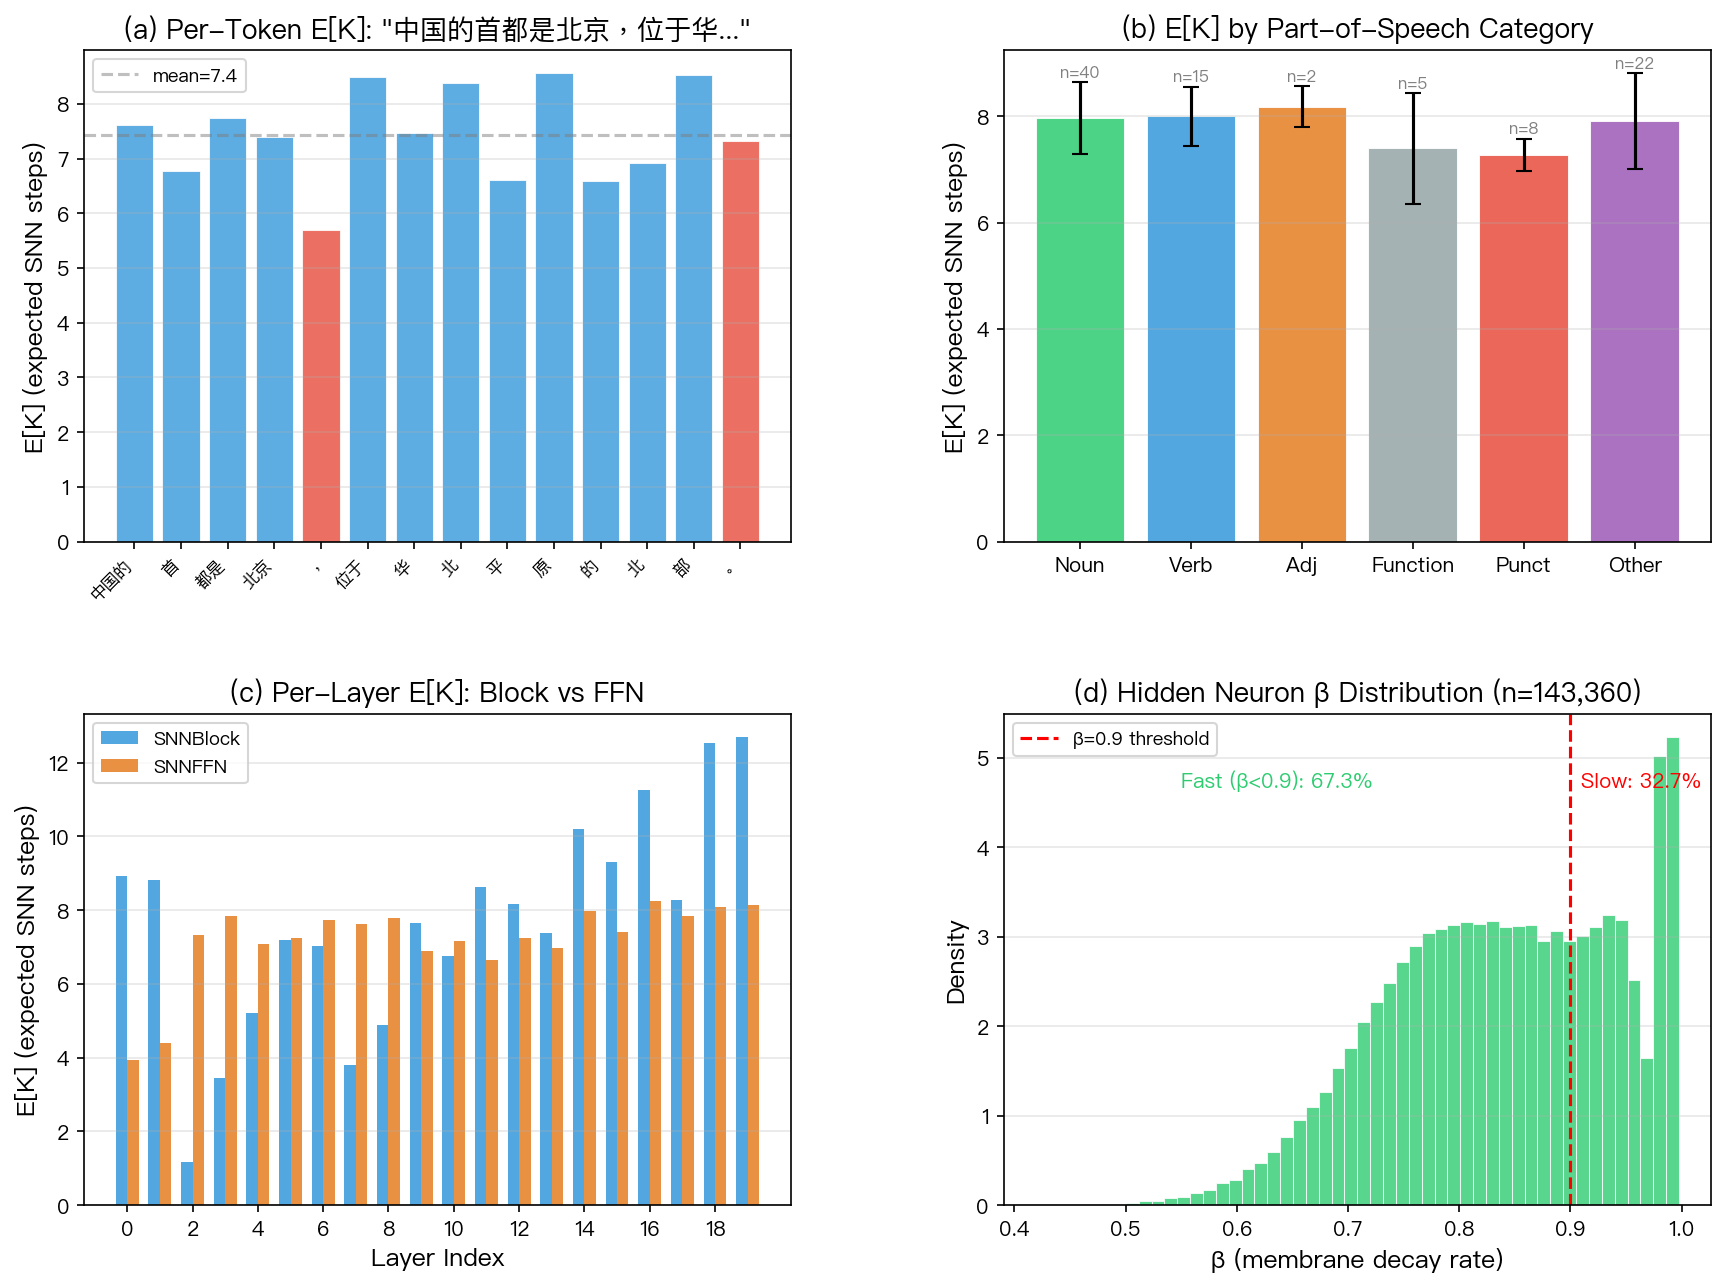
\includegraphics[width=\textwidth]{figures/interpretability.png}
    \caption{Biological interpretability analysis of \model{}-0.9B-Chat on Chinese text (token labels shown in pinyin transliteration).
    \textbf{(a)}~Per-token E[K] for the sentence ``The capital of China is Beijing, located in the northern part of the North China Plain''; punctuation tokens (red) receive notably fewer SNN steps than content words.
    \textbf{(b)}~E[K] grouped by part-of-speech category (jieba Chinese POS tagger, 40 test sentences); function words and punctuation allocate $\sim$0.7 fewer steps than nouns, verbs, and adjectives.
    \textbf{(c)}~Per-layer E[K] for SNNBlock vs.\ SNNFFN; Block E[K] increases monotonically in deeper layers (up to 12.7 at L19), while FFN E[K] remains stable around 7--8.
    \textbf{(d)}~Distribution of learned $\beta$ (membrane decay rate) across all 143,360 hidden neurons; 67.3\% are fast-responding ($\beta < 0.9$) and 32.7\% are slow-memory neurons.}
    \label{fig:interpretability}
\end{figure}

\paragraph{Computation allocation is structural, not predictive.}
A natural hypothesis is that PonderNet allocates more SNN steps to tokens that are harder to predict (high surprisal $= -\log P(\text{next token})$).
Figure~\ref{fig:surprisal} tests this directly on 541 tokens (40 sentences).
Na\"ively, surprisal and E[K] appear negatively correlated ($r = -0.50$); however, this is entirely driven by the BOS (beginning-of-sequence) sentinel token, which has extremely low E[K] (3.2) and high surprisal (8.9) by construction.
Excluding BOS tokens, the correlation drops to $r = -0.12$ (near zero), and binned analysis confirms that mean E[K] is essentially flat ($\sim$7.4--7.9) across all surprisal ranges.

This reveals that \textbf{PonderNet's computation budget is governed by structural/syntactic role rather than predictive difficulty}: punctuation and function words receive fewer steps not because they are easy to predict, but because they play a structurally simpler role in the sequence.
This is consistent with biological findings that neural processing effort correlates more with syntactic complexity than with statistical predictability~\citep{neftci2019surrogate}.

\begin{figure}[H]
    \centering
    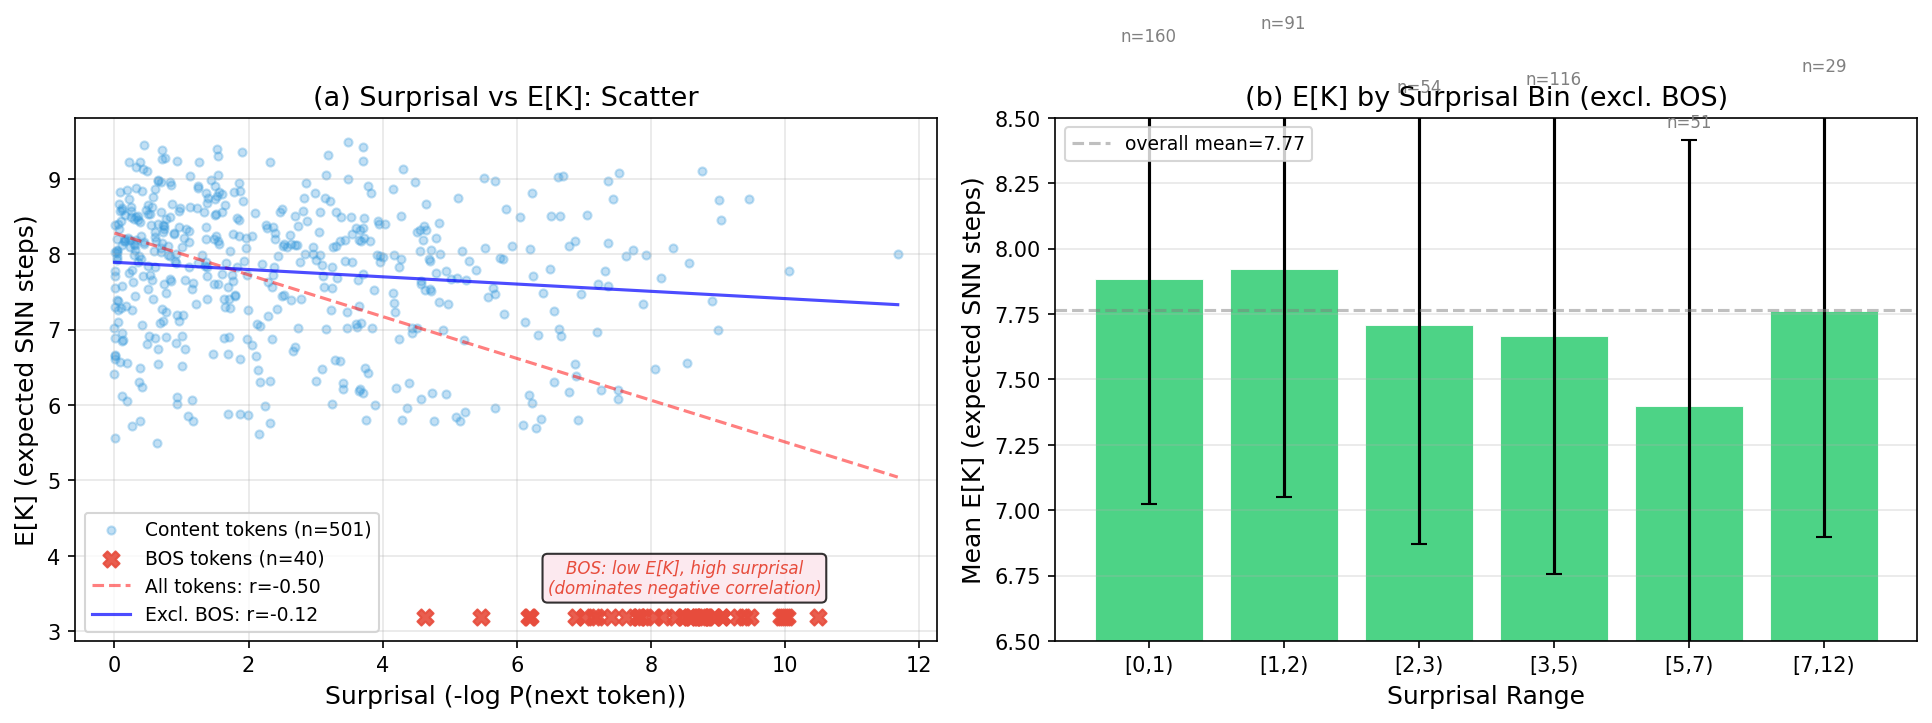
\includegraphics[width=\textwidth]{figures/surprisal_vs_ek.png}
    \caption{Surprisal vs.\ E[K] analysis (40 Chinese sentences, 541 tokens).
    \textbf{(a)}~Scatter plot: BOS tokens (red crosses) dominate the apparent negative correlation ($r{=}{-}0.50$); excluding them yields $r{=}{-}0.12$ (blue line).
    \textbf{(b)}~Mean E[K] binned by surprisal range (excluding BOS): E[K] is flat across all bins, confirming that computation allocation is independent of predictive difficulty.}
    \label{fig:surprisal}
\end{figure}

\paragraph{Reasoning capability assessment.}
To further characterize what the model has and has not learned, we test on 28 questions across four categories: arithmetic (8), logical reasoning (6), commonsense (8), and dialogue coherence (6).
Figure~\ref{fig:reasoning} summarizes the results.

The model achieves \textbf{0\% on arithmetic} (unable to perform any calculation), \textbf{25\% on commonsense} (mostly coincidental keyword matches), and \textbf{83\% on logic} (though inspection reveals many ``correct'' answers arise from the expected keyword appearing in repetitive output rather than genuine inference).
By contrast, \textbf{all 6 coherence tests produce fluent, grammatical Chinese responses}, confirming that the model has acquired surface-level language generation ability.

Critically, panel~(b) shows that \textbf{E[K] is flat ($\sim$7.6) across all categories}, regardless of task difficulty.
The model does not allocate additional SNN computation for harder reasoning tasks, further confirming that PonderNet's adaptive computation is driven by structural token properties (Section~\ref{sec:leakage}) rather than semantic reasoning demands.

These results are consistent with the limited training budget: the model has learned structural language patterns (fluency, POS-dependent computation) but has not yet acquired the factual knowledge or compositional reasoning that would require substantially more training data.

\begin{figure}[H]
    \centering
    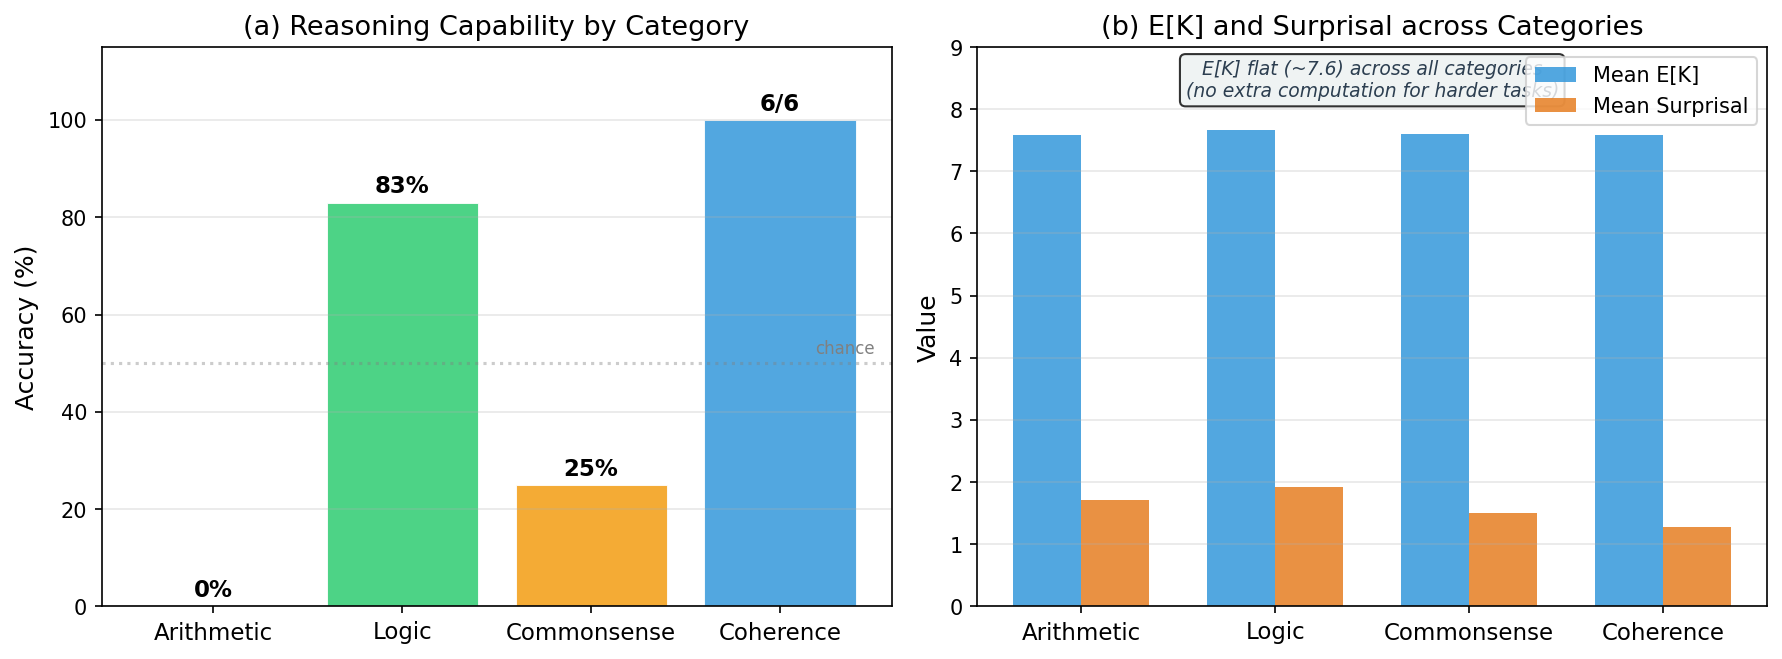
\includegraphics[width=\textwidth]{figures/reasoning_test.png}
    \caption{Reasoning capability assessment (28 questions).
    \textbf{(a)}~Accuracy by category: arithmetic 0\%, logic 83\% (superficial), commonsense 25\%, coherence 6/6.
    \textbf{(b)}~E[K] and surprisal are flat across categories, indicating no adaptive computation increase for harder tasks.
    The model has learned structural language patterns but not reasoning.}
    \label{fig:reasoning}
\end{figure}

\paragraph{Adaptive computation aligns with linguistic complexity.}
Panel~(a) shows that PonderNet assigns systematically fewer SNN timesteps to punctuation (E[K]$\approx$5.7) and function words (E[K]$\approx$7.4) than to content words (nouns 8.0, verbs 8.0, adjectives 8.2).
This pattern --- emerging without any explicit linguistic supervision --- mirrors the intuition that structurally predictable tokens require less neural computation.
The BOS token receives the fewest steps (E[K]=3.2), consistent with it being a fixed sentinel requiring no contextual processing.

\paragraph{Depth-dependent computation budget.}
Panel~(c) reveals a striking asymmetry: SNNBlock E[K] increases monotonically with layer depth (from $\sim$4 at layer~2 to $\sim$12.7 at layer~19), while SNNFFN E[K] remains relatively flat ($\sim$7--8).
This suggests that deeper layers require more SNN timesteps for the attention-analogue computation (SNNBlock) but not for the feed-forward transformation (SNNFFN).
A possible interpretation is that deeper layers perform more complex contextual integration, requiring longer membrane-potential evolution, while the point-wise nonlinear transformation in SNNFFN saturates at a fixed computation depth.

\paragraph{Multi-timescale neuron specialization.}
Panel~(d) shows that the 143,360 hidden neurons self-organize into fast-responding ($\beta < 0.9$, 67.3\%) and slow-memory ($\beta \geq 0.9$, 32.7\%) populations.
This is reminiscent of biological cortical circuits where fast-spiking interneurons coexist with regular-spiking pyramidal cells operating at different timescales.
The distribution is unimodal with a long right tail, indicating that the model learns a continuum of timescales rather than a sharp dichotomy, with a preference for faster dynamics.

\end{document}
